\documentclass{article}
\usepackage[utf8]{inputenc}
% important for graphicx
\usepackage{graphicx}
\graphicspath{{img/}{src/}}
\usepackage{float}
\usepackage{hyperref}
\usepackage{enumitem}
\usepackage{algorithm}
\usepackage{subcaption}
\usepackage[mathscr]{euscript}
\usepackage[detect-all]{siunitx}
\usepackage[noend]{algpseudocode}
% background color for definitions
\usepackage[most]{tcolorbox}
\tcbset{
    frame code={}
    center title,
    left=0pt,
    right=0pt,
    top=0pt,
    bottom=0pt,
    colback=blue!6!white,
    colframe=white,
    width=\dimexpr\textwidth\relax,
    enlarge left by=0mm,
    boxsep=10pt,
    arc=0pt,outer arc=0pt,
}

\newenvironment{changemargin}[2]{%
\begin{list}{}{%
\setlength{\topsep}{0pt}%
\setlength{\leftmargin}{#1}%
\setlength{\rightmargin}{#2}%
\setlength{\listparindent}{\parindent}%
\setlength{\itemindent}{\parindent}%
\setlength{\parsep}{\parskip}%
}%
\item[]}{\end{list}}

\usepackage{listings}
\usepackage{xcolor}

%New colors defined below
\definecolor{codegreen}{rgb}{0,0.6,0}
\definecolor{codegray}{rgb}{0.5,0.5,0.5}
\definecolor{codepurple}{rgb}{0.58,0,0.82}
\definecolor{backcolour}{rgb}{0.95,0.95,0.92}

%Code listing style named "mystyle"
\lstdefinestyle{mystyle}{
  backgroundcolor=\color{backcolour},   commentstyle=\color{codegreen},
  keywordstyle=\color{magenta},
  numberstyle=\tiny\color{codegray},
  stringstyle=\color{codepurple},
  basicstyle=\ttfamily\footnotesize,
  breakatwhitespace=false,         
  breaklines=true,                 
  captionpos=b,                    
  keepspaces=true,                 
  numbers=left,                    
  numbersep=5pt,                  
  showspaces=false,                
  showstringspaces=false,
  showtabs=false,                  
  tabsize=2
}

%"mystyle" code listing set
\lstset{style=mystyle}

\title{Code Listing}
\date{ }

\begin{document}

\title{Image Processing III\\
Mutual Information}
\author{Aadil Anil Kumar \\
Otmane Sabir
}
\date{26/4/2020}
\maketitle
\vspace{10mm}
\begin{center}
\section*{Introduction}
\large
The third homework assignment required us to implement the similarity metric algorithm "mutual information" while following certain guidelines which could be summarized to the following list: 
\vspace{7mm}
\begin{enumerate}
    \item Implement the algorithm.
    \item Choose 3 images from the internet and separate the green and red channels as two separate gray scale images each. Crop the green channel by cutting 20 pixels from the left and right sides, respectively - resulting in a cropped green channel image with 40 pixels smaller than the red channel image. Then virtually move the red channel images in x-direction over the corresponding green channel image in 41 steps from the left to right, and compute the mutual information of the overlapping regions for every step.
    \item Plot the mutual information as a function of the x-position of the red channel image for all three chosen red/green image pairs.
\end{enumerate}


\end{center}
\newpage

\tableofcontents

\newpage

\section{Mutual Information}
\vspace{2mm}
\begin{flushleft}
Mutual information is a quantity that measures a relationship between two random variables that are sampled simultaneously. In particular, it measures how much information is communicated, on average, in one random variable about another. For example, suppose X represents the roll of a fair 6-sided die, and Y represents whether the roll is even (0 if even, 1 if odd). Clearly, the value of Y tells us something about the value of X and vice versa. That is, these variables share mutual information. \cite{entropy&mi}
\end{flushleft}
\vspace{2mm}
\begin{figure}[ht]
    \centering
    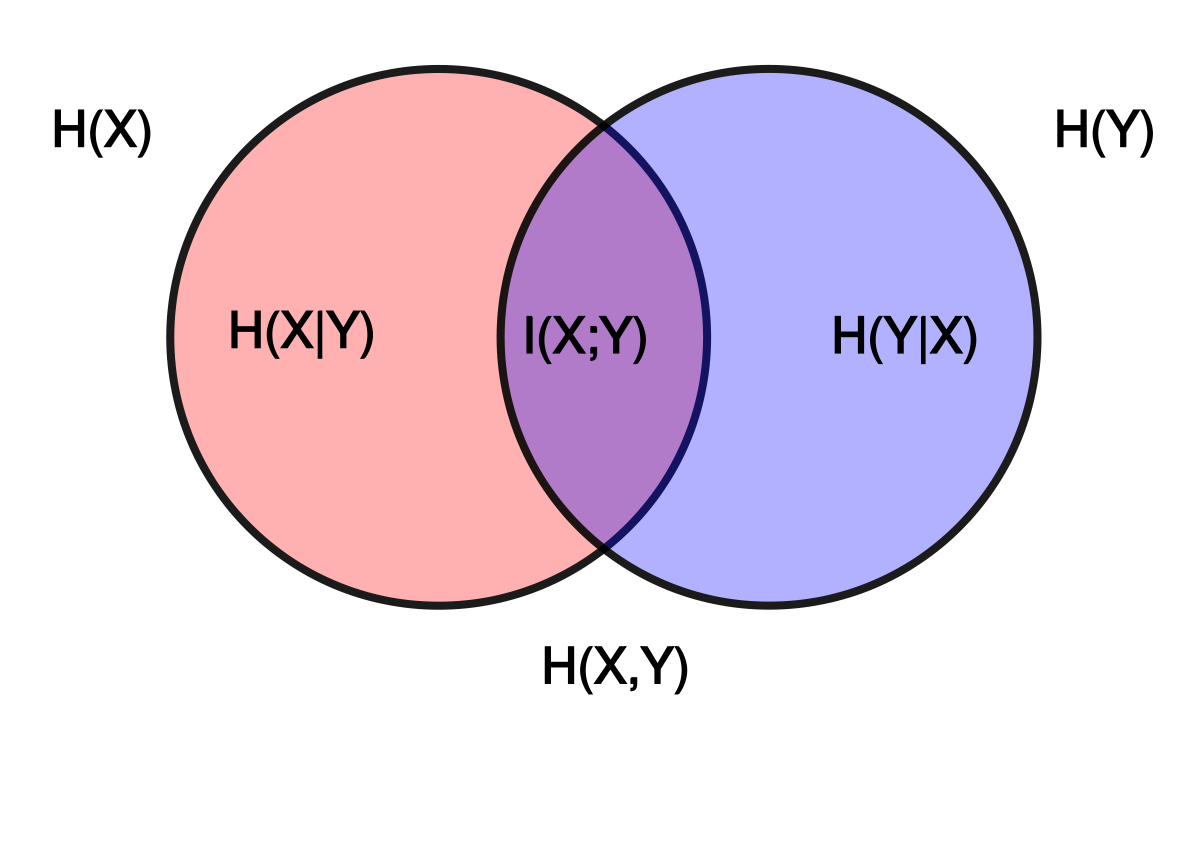
\includegraphics[width=\linewidth]{mutual information.png}
    \caption{Mutual Information Visualization}
    \label{fig:watershed_visualization}
\end{figure}

\subsection{Formal Definition}
\begin{flushleft}
\vspace{2mm }
\begin{tcolorbox}
\textsc{Definition:}\cite{wiki}\cite{quantiki}\newline\newline
The formal definition of the mutual information of two random variables $X$ and $Y$, whose joint distribution is defined by $P(X, Y)$ is given by
\vspace{4mm}
\begin{center}
\[
I(X;Y) = \sum_{x \in X}^{}\sum_{y \in Y}^{} P(x, y)\log \frac{P(x, y)}{P(x)P(y)}
\]
\end{center}
Such that, $P(X)$ and $P(Y)$ are the \textit{marginal distributions} of $X$ and $Y$ obtained through the marginalization process which can be defined as : 
\begin{center}
\[
p_X(x_i) = \sum_{j}p(x_i, y_i)
\]

\[
p_Y(y_j) = \sum_{i}p(x_i, y_i) 
\]
\end{center}
\end{tcolorbox}
\end{flushleft}

\section{Shannon Entropy \& Mutual Information}
\vspace{2mm}
\begin{flushleft}
In our implementation, we rely on calculating the shannon entropy in order to estimate the mutual information. Intuitively, some may ask what is entropy? 
\end{flushleft}
The entropy is the expected value of the self-information, the self-information quantifies the level of information or surprise associated with one particular outcome or event of a random variable, whereas the entropy quantifies how "informative" or "surprising" the entire random variable is, averaged on all its possible outcomes.

\subsection{Formal Definition : Shannon Entropy}
\label{marker}
\vspace{2mm}
\begin{flushleft}
\vspace{2mm }
\begin{tcolorbox}
\textsc{Definition:}\cite{wiki-shannon}\newline\newline
The formal definition of the entropy of a discrete random variable $X$ with possible values $\{x_1, ... ,x_n\}$ and probability mass function $P(X)$ is
\vspace{4mm}
\begin{center}
\[
H(X) = - \sum{P(x_i)\log_b P(x_i)}
\]
\end{center}
\vspace{4mm}
where $b$ is the base of the logarithm used. Common values of b are 2, Euler's number $e$, and 10. In the case of $P(x_i) = 0$ for some $i$, the value of the corresponding summand $0\log_b (0)$ is taken to be 0.
\end{tcolorbox}
\end{flushleft}

\subsection{Formal definition : Mutual Information}
\label{marker2}
\vspace{2mm}
\begin{flushleft}
\vspace{2mm}
\begin{tcolorbox}
\textsc{Definition:}\cite{quantiki}\newline\newline
If we consider pairs of discrete random variables (X,Y), then formally, the mutual information can be defined as :
\begin{center}
\[
I(X : Y) = H(X) + H(Y) - H(XY)
\]
\end{center}
\vspace{2mm}
with $H(X)$, $H(Y)$ the Shannon entropy of $X$ an $Y$, and $H(XY)$ the Shannon entropy of the pair $(X, Y)$. 
\end{tcolorbox}
\end{flushleft}

\section{Implementation}
\vspace{2mm}
\begin{flushleft}
We decided to implement our algorithm in python for ease of implementation and the support provided from preexisting libraries. We first started by implementing a simple entropy computation method, then by interpreting the image signals from the image to match our entropy function and then applying the formula from the previous definition.

Before we start implementing, this is a list of all libraries and styles used in order to calculate, convert and plot our results.
\end{flushleft}
\begin{lstlisting}[language=Python]
import numpy as np
import matplotlib.pyplot as plt
import seaborn as sns
from scipy.stats import entropy as scipy_entropy
from PIL import Image
plt.style.use('seaborn')
\end{lstlisting}

\subsection{Entropy function :}
\vspace{2mm}
\begin{flushleft}
This is a simple implementation of the entropy function. Given the input parameter $X$ which in our case is a random variable, we get the entropy of the random variable. In subsection \textbf{\ref{marker}} we introduced a formal definition of this calculation.
\end{flushleft}
\begin{lstlisting}[language=Python, caption=Entropy Calculator]
def entropyCalc(X):
    uniq = set(X)
    P = [np.mean(X == x) for x in uniq]
    return sum(-p * np.log2(p) for p in P)

\end{lstlisting}

\subsection{Converting the image}
\vspace{2mm}
\begin{flushleft}
In order for our entropy function to properly compute these values we need to convert the image from the matrices we receive to appropriate signals. We do this by using the numpy histogram functions in the case of the join histogram.
\end{flushleft}
\begin{lstlisting}[language=Python, caption=1D Signal]
def convert1DSignal(x, nBins):
    return np.histogram(np.asarray(x).flatten(), bins=nBins)[0]
\end{lstlisting}

\begin{lstlisting}[language=Python, caption=2D Signal (Joint Histogram)]
def convert2DSignal(x, y, nBins):
    hist = np.histogram2d(np.asarray(x).flatten(), np.asarray(y).flatten(), bins=nBins)
    return np.asarray(Image.fromarray(hist[0], 'RGB')).flatten()
\end{lstlisting}

\subsection{Mutual Information}
\begin{flushleft}
We now have all the required tools to calculate our mutual information estimation. The mutual information function will be very simple and will follow our definition in the subsection \textbf{\ref{marker2}}.
\end{flushleft}

\begin{lstlisting}[language=Python, caption=Mutual Information]
def mutualInformation(x, y, nBins):
    HX = entropyCalc(convert1DSignal(x, nBins))
    HY = entropyCalc(convert1DSignal(y, nBins))
    HXY = entropyCalc(convert2DSignal(x, y, nBins))
    return HX + HY - HXY
\end{lstlisting}

\section{Experiments \& Results}

\begin{flushleft}
The experiments we were asked to conduct were an intuitive way of visualizing how mutual information exactly works. We were asked to choose 3 images from the internet and separate the green and red channels as two separate gray scale images each. Crop the green channel by cutting 20 pixels from the left and right sides, respectively - resulting in a cropped green channel image with 40 pixels smaller than the red channel image. Then virtually move the red channel images in x-direction over the corresponding green channel image in 41 steps from the left to right, and compute the mutual information of the overlapping regions for every step and then finally plot the mutual information as a function of the x-position of the red channel image for all three chosen red/green image pairs.
\end{flushleft}

\subsection{Puffin Experiment}
\newpage

\begin{thebibliography}{9}
\label{sec:hello}

\bibitem{entropy&mi}
Entropy and Mutual Information: \newline
AS Kornillov
\\\texttt{https://people.cs.umass.edu/~elm/Teaching/Docs/mutInf.pdf}

\bibitem{wiki}
Mutual Information: \newline
Wikipedia 
\\
\texttt{https://en.wikipedia.org/wiki/Mutual_information}

\bibitem{quantiki}
Mutual Information : \newline
Quantiki :
\\
\texttt{https://www.quantiki.org/wiki/mutual-information}

\bibitem{wiki-shannon}
Entropy (Information Theory) : \newline
Wikipedia :
\\
\texttt{https://en.wikipedia.org/wiki/Entropy_(information_theory)}

\end{thebibliography}

\end{document}
